\documentclass[lettersize,journal]{IEEEtran}
\usepackage{amsmath,amsfonts}
\usepackage{array}
\usepackage[caption=false,font=normalsize,labelfont=sf,textfont=sf]{subfig}
\usepackage{textcomp}
\usepackage{stfloats}
\usepackage{url}
\usepackage{verbatim}
\usepackage{graphicx}
\usepackage{cite}
\graphicspath{{Figures/}}
\hyphenation{op-tical net-works semi-conduc-tor IEEE-Xplore}

\begin{document}

\title{A Survey on RRAM Technology and MOS Integration}

\author{Ashton~Billings and Jack~Walberer%
\thanks{A.~Billings and J.~Walberer are with the Department of Electrical and Computer Engineering, University of Illinois Urbana--Champaign, Urbana, IL 61801 USA (e-mail: ashtonrb1@gmail.com).}%
\thanks{Manuscript prepared for ECE~585 (MOS Device Modeling), Spring 2026.}}

\markboth{ECE~585 Term Project, Spring~2026}%
{Billings and Walberer: A Survey on RRAM Technology and MOS Integration}

\maketitle

\begin{abstract}
Resistive random-access memory (RRAM) is the leading candidate to replace embedded flash at logic nodes below 28~nm, where the floating-gate stack no longer scales. This survey reviews the device, its dominant operating mechanism, and how it is integrated into modern CMOS. The metal--insulator--metal (MIM) cell and the standard taxonomy of resistive switching are first introduced. Among the available switching mechanisms, the industry has converged on the valence-change mechanism (VCM) using HfO\textsubscript{2} or TaO\textsubscript{x} as the switching oxide. The cell is then placed in its production context: a 1-transistor--1-resistor (1T1R) configuration in which a CMOS MOSFET sets the compliance current, addresses the cell, and isolates unselected cells from sneak-path leakage. The select-FET design problem is examined explicitly, including a worked sizing example on a 0.25~$\mu$m planar process from the literature, and the constraints are tracked across the planar bulk, FD-SOI, and FinFET architectures that host RRAM in industry today.
\end{abstract}

\begin{IEEEkeywords}
Resistive random-access memory, RRAM, ReRAM, valence-change mechanism, oxygen vacancy, HfO\textsubscript{2}, TaO\textsubscript{x}, embedded non-volatile memory, 1T1R, 1-transistor 1-resistor, BEOL integration, FinFET, FD-SOI.
\end{IEEEkeywords}

\section{Introduction}
\IEEEPARstart{F}{or} more than two decades, embedded flash (eFlash) has served as the default non-volatile memory in microcontrollers, automotive ICs, and IoT system-on-chips. Its physical foundation---a floating-gate or charge-trap MOSFET that retains charge across a tunnel oxide of roughly 7--10~nm---is incompatible with logic scaling: retention specifications fix a minimum oxide thickness that does not shrink with the logic node, and the supporting high-voltage charge pumps add significant mask count and process complexity. By the time the industry reached the 28~nm node, eFlash had become a process integration burden that foundries were no longer willing to carry forward, and TSMC publicly stopped offering eFlash beyond 28~nm in the late 2010s~\cite{ref_hellenbrand2024}. The resulting gap created the commercial opening for emerging non-volatile memories.

Among the emerging candidates, resistive RAM (RRAM) is attractive because its cell is a simple two-terminal metal--insulator--metal (MIM) stack of materials already qualified in CMOS fabrication, it is built in the back-end-of-line (BEOL) above the transistors, and its mask adder is small. The cell does not stand alone; in production it is paired with a select MOSFET in a 1-transistor--1-resistor (1T1R) configuration, which makes the technology directly relevant to MOSFET device modeling.

This survey is organized around four questions, mirroring the project presentation. Section~\ref{sec:what} introduces the RRAM cell and the family of resistive switching mechanisms, focusing on the valence-change mechanism (VCM) that dominates today's commercial cells. Section~\ref{sec:why} addresses why RRAM is being adopted, where it fits in the memory hierarchy, and where it currently sits in industry. Section~\ref{sec:how} treats the integration of the cell into CMOS through the 1T1R architecture and the select-FET sizing problem, with a worked example on a planar process. Section~\ref{sec:tech} compares the three MOSFET architectures---planar bulk, FD-SOI, and FinFET---that host RRAM at production nodes. Section~\ref{sec:conclusion} concludes.

\section{What is RRAM?}\label{sec:what}

\subsection{The RRAM Cell}
RRAM is a form of non-volatile memory in which information is stored in the resistance of a two-terminal device~\cite{ref_waser2009,ref_wong2012}. A high-resistance state (HRS) is read as logic~0 and a low-resistance state (LRS) is read as logic~1. The transition from HRS to LRS is called SET, and the reverse transition is RESET. Because the storage element is a passive resistor rather than a charge-storing capacitor, RRAM does not suffer from the tunnel-oxide thickness floor that limits flash scaling.

In an array, the resistive switching element (RS) is paired with a non-linear element (NLE) that selects which cell is being addressed. The two canonical choices for the NLE are a two-terminal selector and a CMOS MOSFET, shown in Fig.~\ref{fig_cell_choices}. The MOSFET-based 1T1R cell on the right is the configuration used in essentially every embedded RRAM product shipping today, because the MOSFET simultaneously addresses the cell, sets the compliance current during programming, and blocks leakage from unselected cells during read~\cite{ref_waser2009,ref_ielmini2016}.

\begin{figure}[!t]
\centering

\includegraphics[width=2.2in]{fig1.png}
\caption{RRAM cell architectures. (a)~Selector-based cell, in which a two-terminal non-linear element (NLE) is placed in series with the resistive switch (RS). (b)~1T1R cell, in which a CMOS MOSFET serves as the select element. Reproduced from~\cite{ref_waser2009}.}
\label{fig_cell_choices}
\end{figure}

\subsection{Resistive Switching Mechanisms}
Many physical mechanisms can produce a reversible resistance change in a thin film. Waser~\textit{et~al.} organize the field into the taxonomy reproduced in Fig.~\ref{fig_taxonomy}, which spans nanomechanical, molecular, electrostatic/electronic, electrochemical metallization, valence-change, thermochemical, phase-change, magnetoresistive, and ferroelectric tunneling effects~\cite{ref_waser2009}. The right-hand axis classifies each mechanism by the dominant species (electrode-dominated vs.~chalcogenide-dominated, redox-related) and by switching polarity (unipolar vs.~bipolar). Of the redox-based mechanisms, three are most relevant to memory.

\begin{figure}[!t]
\centering
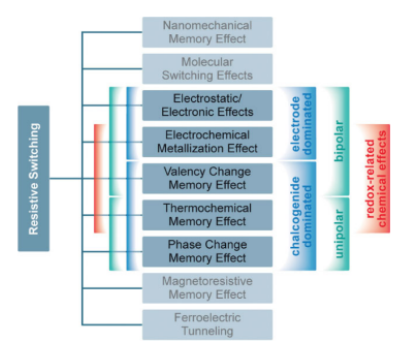
\includegraphics[width=2.4in]{fig2.png}
\caption{Taxonomy of resistive switching mechanisms. Reproduced from~\cite{ref_waser2009}.}
\label{fig_taxonomy}
\end{figure}

\textit{Electrochemical Metallization Mechanism (ECM).} An electrochemically active electrode (typically Ag or Cu) dissolves under positive bias, drifts through a solid electrolyte, and electrocrystallizes into a metallic filament that bridges the electrodes~\cite{ref_waser2009}. ECM operates at very low voltages but the metallic filament is sensitive to thermal activation, which complicates retention.

\textit{Thermochemical Mechanism (TCM).} Switching is driven by Joule heating, with SET and RESET at the same polarity but different current levels (unipolar). NiO is the canonical TCM material~\cite{ref_waser2009}. TCM has lost commercial relevance because each RESET is essentially a controlled local meltdown of the filament, and cycle-to-cycle variability is intractable.

\textit{Valence-Change Mechanism (VCM).} The mobile species is the oxygen anion (or, equivalently, the oxygen vacancy~$V_\mathrm{O}$). Under field, oxygen drifts away from a region of the oxide, leaving an oxygen-deficient sub-stoichiometric path of higher conductivity. Because metal cations along the path are reduced to a lower oxidation state (e.g., Hf$^{4+}\!\rightarrow\!$Hf$^{3+}$, Ta$^{5+}\!\rightarrow\!$Ta$^{4+}$), the mechanism takes its name from this valence change~\cite{ref_waser2009}. Reversing the bias drives oxygen back. VCM is bipolar and is the family that includes HfO\textsubscript{x} and TaO\textsubscript{x} RRAM~\cite{ref_wong2012,ref_ielmini2016}.

The industry has converged on VCM, with HfO\textsubscript{2} and TaO\textsubscript{x} as the two switching oxides that have crossed into foundry production~\cite{ref_wong2012,ref_hellenbrand2024}. HfO\textsubscript{2} is already qualified as the high-$\kappa$ gate dielectric in modern HKMG MOSFETs, which makes it especially attractive: deposition equipment, contamination protocols, and reliability physics are already characterized in the fab. TaO\textsubscript{x} systems achieve higher endurance than HfO\textsubscript{x} in optimized lab structures, and TaO\textsubscript{x}-based ReRAM has been commercialized by Weebit~Nano in partnership with GlobalFoundries (22FDX) and SkyWater (130~nm)~\cite{ref_hellenbrand2024}.

\subsection{How VCMs Work}
A VCM cell is a passive MIM stack: a transition-metal oxide a few nanometers thick is sandwiched between a top electrode and a bottom electrode (Fig.~\ref{fig_mim}). When a voltage is applied, oxygen ions and oxygen vacancies migrate through the oxide and reorganize into a conductive filament that connects the two electrodes. Reversing or reducing the applied bias partially disconnects the filament, returning the cell to a high-resistance state~\cite{ref_wong2012,ref_ielmini2016}.

\begin{figure}[!t]
\centering
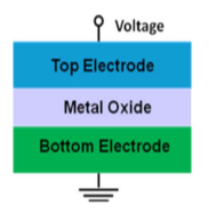
\includegraphics[width=1.2in]{fig3.png}
\caption{The metal--insulator--metal (MIM) cell stack. A thin transition-metal oxide is sandwiched between two metal electrodes. Reproduced from~\cite{ref_wong2012}.}
\label{fig_mim}
\end{figure}

The full SET/RESET cycle is shown in Fig.~\ref{fig_cycle}. In the as-fabricated state the oxide is essentially an insulator (initial resistance state, IRS). A one-time soft dielectric breakdown step, called \textit{forming} or \textit{electroforming}, is required to nucleate the conductive filament~\cite{ref_wong2012}. During forming a voltage larger than the operational SET voltage is applied while the current is held to a compliance level $I_\mathrm{CC}$, typically by a series transistor. The compliance current is essential because it limits the energy delivered into the dielectric and prevents an irreversible hard breakdown. After forming, the cell can be cycled at lower voltage between SET (HRS$\rightarrow$LRS, soft breakdown that reconnects the filament) and RESET (LRS$\rightarrow$HRS, partial rupture of the filament). In bipolar operation the SET and RESET pulses have opposite polarity; in unipolar operation they share polarity but differ in current level~\cite{ref_wong2012,ref_waser2009}.

\begin{figure}[!t]
\centering
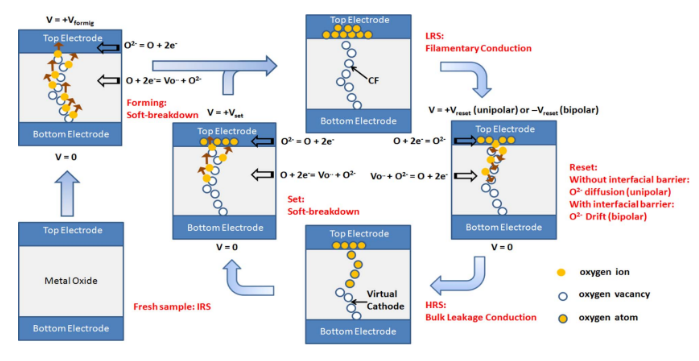
\includegraphics[width=3.4in]{fig4.png}
\caption{Operation of a VCM cell. Starting from the as-fabricated insulating state, a forming pulse nucleates a conductive filament of oxygen vacancies. Subsequent SET pulses reconnect the filament to enter the LRS; RESET pulses partially rupture the filament to return to the HRS. Reproduced from~\cite{ref_wong2012}.}
\label{fig_cycle}
\end{figure}

In the LRS, conduction is approximately ohmic and dominated by the metallic-like sub-stoichiometric filament. In the HRS, conduction is more complex and depends on the material system: trap-assisted tunneling, Poole--Frenkel emission, and Schottky emission at the oxide/electrode interface have all been reported~\cite{ref_wong2012}. The result is a non-trivial $I$--$V$ shape that depends on electrode work function, oxide stoichiometry, and process conditions.

\section{Why RRAM?}\label{sec:why}

\subsection{The eFlash Replacement Argument}
The first and primary commercial driver for RRAM is the replacement of embedded flash at advanced nodes. Embedded flash does not scale below approximately 28~nm: the tunnel oxide cannot be thinned without sacrificing 10-year retention, and the high-voltage charge pumps required to program the cell add area and mask count that grow as a fraction of the die at advanced nodes~\cite{ref_hellenbrand2024}. RRAM avoids both problems. The MIM cell stack is on the order of 5--10~nm thick and does not rely on charge storage, so retention is governed by the thermal stability of the oxygen-vacancy distribution rather than by tunnel-oxide leakage. Programming voltages, while higher than core-logic $V_\mathrm{DD}$, are an order of magnitude below those required for flash, which makes the on-die charge pump correspondingly smaller~\cite{ref_wong2012,ref_hellenbrand2024}.

A second advantage is back-end-of-line (BEOL) integration. The MIM stack is fabricated in the metal layers above the transistors, between two interconnect levels. The front-end logic flow is essentially unchanged, and the memory module adds only one or two extra masks~\cite{ref_wong2012}. This stands in sharp contrast to embedded flash, which requires its own front-end module. BEOL integration also enables stacking, which gives RRAM a path toward higher density that planar charge-storage memories do not have.

A third, more speculative possibility is that the same simplicity that lets RRAM displace eFlash could eventually let it displace volatile memories such as SRAM and DRAM in some workloads, particularly those dominated by infrequent writes and large read-mostly state~\cite{ref_wong2012}.

\subsection{Industry Adoption}
By the mid-2020s embedded RRAM is a foundry-process option at multiple companies. Fig.~\ref{fig_industry} reproduces the industry timeline assembled by Hellenbrand~\textit{et~al.} for FRAM, MRAM, PCRAM, and RRAM from 2017 through 2026~\cite{ref_hellenbrand2024}. RRAM has the densest population in the chart, with announcements from TSMC, UMC, Fujitsu, Infineon, Microsemi, Intel, Weebit~Nano (with GlobalFoundries), and others.

\begin{figure*}[!t]
\centering
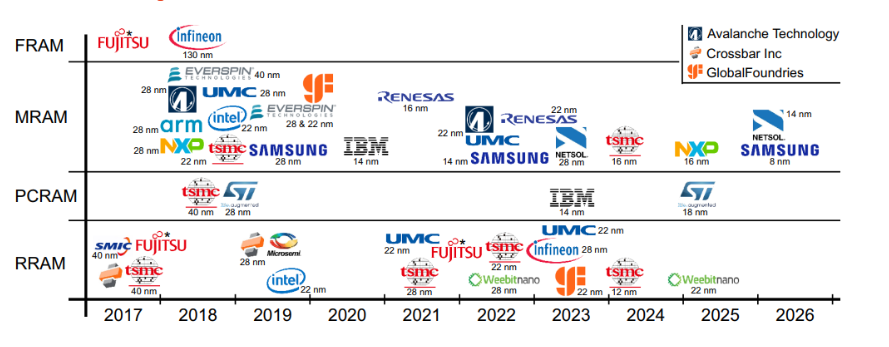
\includegraphics[width=6.5in]{fig5.png}
\caption{Industry roadmap for emerging non-volatile memories from 2017 through 2026. RRAM has the densest set of announcements among the four families. Reproduced from~\cite{ref_hellenbrand2024}.}
\label{fig_industry}
\end{figure*}

The dominant players, with the most representative recent announcements, are:
\begin{itemize}
\item \textit{TSMC.} HfO\textsubscript{2}-based embedded RRAM at 40~nm, 28~nm, and 22~nm planar bulk, with a 12~nm FinFET demonstration presented at IEDM~2023~\cite{ref_hellenbrand2024}.
\item \textit{Intel.} A 22~nm FinFET RRAM cell using a TaO\textsubscript{x}-based switching oxide~\cite{ref_hellenbrand2024}.
\item \textit{IBM.} Investigating both TaO\textsubscript{x} and HfO\textsubscript{2} stacks for analog in-memory compute, exploiting the continuous conductance levels available in VCM cells~\cite{ref_hellenbrand2024}.
\end{itemize}

The applications are nearly exclusively embedded: firmware code, calibration constants, AI inference weights, and secure keys in microcontrollers, automotive ICs, IoT system-on-chips, and secure elements~\cite{ref_hellenbrand2024}. What unifies these workloads is that writes are infrequent (often write-once at provisioning), retention requirements are stringent, and security or latency forbids using an external SPI flash chip.

\subsection{Position in the Memory Hierarchy}
A useful way to see RRAM's niche is to place it directly against the dominant memory technologies. Table~\ref{tab:memory_compare} summarizes the comparison.

\begin{table}[!t]
\caption{Comparison of RRAM and Conventional Memory Technologies\label{tab:memory_compare}}
\centering
\footnotesize
\renewcommand{\arraystretch}{1.2}
\begin{tabular}{|p{0.85in}|p{0.42in}|p{0.42in}|p{0.5in}|p{0.45in}|p{0.5in}|}
\hline
 & \textbf{SRAM} & \textbf{DRAM} & \textbf{Flash NAND} & \textbf{Flash NOR} & \textbf{RRAM} \\
\hline
Volatile? & Volatile & Volatile & Non-vol. & Non-vol. & Non-vol. \\
\hline
Cell size & $\sim$50~$F^2$ & $\sim$6~$F^2$ & $\sim$4~$F^2$ & $\sim$10~$F^2$ & $\sim$6--12~$F^2$ \\
\hline
Read speed & Fast & Fast & Slow & Fast & Fast \\
\hline
Write speed & Fast & Fast & Slow & Slow & Medium \\
\hline
Endurance & Unlimited & $\sim$$10^{15}$ & $10^4$--$10^5$ & $10^4$--$10^5$ & $10^6$--$10^9$ \\
\hline
Write voltage & $V_\mathrm{DD}$ & $V_\mathrm{DD}$ & $\sim$20~V & $\sim$20~V & $V_\mathrm{DD}$+boost $\sim$2~V \\
\hline
Granularity & per-bit & per-bit & block-erase & block-erase & per-bit \\
\hline
On-chip use & Yes & No & No & Yes & Yes \\
\hline
\end{tabular}
\end{table}

The pattern is that RRAM is an embedded non-volatile technology with cell area between DRAM and SRAM, fast read, medium write, per-bit programmability, and a write voltage that requires only a modest on-die boost. Its endurance ($10^6$--$10^9$ cycles) is two to three orders of magnitude better than flash but several orders worse than DRAM, which is why RRAM has not displaced DRAM in working memory. Its niche is precisely the embedded NVM role formerly held by NOR flash, with substantially better scalability and a credible path to denser arrays.

\section{RRAM in CMOS: 1T1R Integration}\label{sec:how}

\subsection{Competing Architectures: 1T1R and the Crossbar}
At the array level there are two competing architectures, illustrated in Fig.~\ref{fig_arch}. In the 1T1R architecture, every cell carries its own select MOSFET, fabricated in the front-end logic flow, with the RRAM stack placed in the BEOL above it~\cite{ref_niu2016}. In the crossbar architecture, the RRAM cells sit at the intersections of orthogonal bitlines and wordlines, with no per-cell select element; addressing relies on biasing the selected lines and the unselected lines at different voltages.

\begin{figure}[!t]
\centering
\subfloat[1T1R]{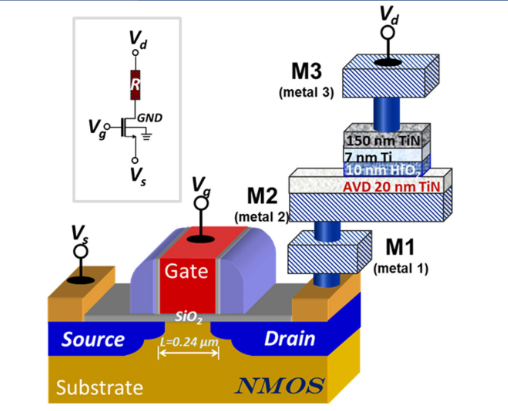
\includegraphics[width=1.7in]{fig7.png}}\hfil
\subfloat[Crossbar]{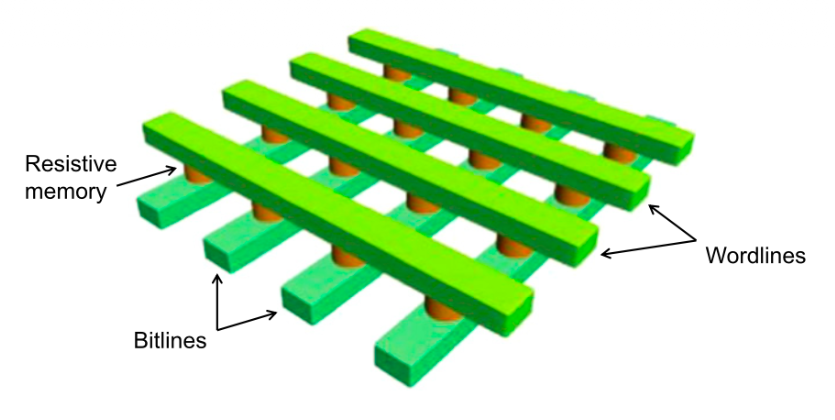
\includegraphics[width=1.5in]{fig8.png}}
\caption{Competing RRAM array architectures. (a)~1T1R: a CMOS NMOS in the front-end with the HfO\textsubscript{2}/Ti/TiN MIM stack between metals~2 and~3. Reproduced from~\cite{ref_niu2016}. (b)~Passive crossbar with bitlines, wordlines, and resistive memory at every intersection. Reproduced from~\cite{ref_ielmini2016}.}
\label{fig_arch}
\end{figure}

The two architectures use very different bias schemes, summarized in Table~\ref{tab:bias}. In 1T1R, the select MOSFET clamps the cell current and isolates unselected rows, so the bias scheme is straightforward: drive the bitline (BL) to the read or write voltage, hold the source line (SL) at ground, and use the wordline (WL) to gate the selected MOSFET into triode (read) or saturation (write). In the crossbar, no transistor is available, so a half-select scheme is used: the selected wordline is biased at $+V_w/2$ and the selected bitline at $-V_w/2$ (or the read variant at $\pm V_r/2$), so that only the targeted intersection sees the full programming voltage. Half-selected cells still see $V_w/2$ across them, however, and the resulting sneak current
\begin{equation}
I_\mathrm{sneak} \;=\; \frac{(N-1)\,V_r}{2\,R_\mathrm{LRS}}
\label{eq:sneak}
\end{equation}
limits the maximum array fan-out $N$ at which the read margin remains acceptable~\cite{ref_ielmini2016}. The crossbar promises a theoretical $4F^2$ cell footprint and a path to true three-dimensional stacking, but only works in production if the sneak current is suppressed by an effective two-terminal selector at every node. No such selector has yet entered foundry production for embedded RRAM, which is why every commercial RRAM macro shipping today is 1T1R.

\begin{table}[!t]
\caption{Bias Schemes for 1T1R and Crossbar Arrays\label{tab:bias}}
\centering
\footnotesize
\renewcommand{\arraystretch}{1.25}
\begin{tabular}{|p{0.42in}|p{1.55in}|p{1.55in}|}
\hline
\textbf{Op.} & \textbf{1T1R} & \textbf{Crossbar} \\
\hline
READ & BL: 0.3--0.4~V; SL:~0~V; WL:~$V_\mathrm{DD}$. MOSFET in triode; sense $I_\mathrm{cell}$ vs.~$I_\mathrm{ref}$; $R_\mathrm{HRS}/R_\mathrm{LRS}\!\sim\!10$--$1000\times$ in HfO\textsubscript{2}. & WL:~$-V_r/2$, BL:~$+V_r/2$. Sneak current $I_\mathrm{sneak}=(N{-}1)V_r/(2R_\mathrm{LRS})$ limits array fan-out. \\
\hline
SET & BL: 2--2.5~V; SL:~0~V; WL:~$V_\mathrm{DD}$. MOSFET in saturation, used to limit sudden current jump; $R_\mathrm{LRS}\!\approx\!V_c/I_\mathrm{cc}$. & WL:~$+V_w/2$, BL:~$-V_w/2$. Cannot limit sudden current jump when channel conducts; $N{-}1$ half-selected cells. \\
\hline
RESET & SL: 1.5~V; BL:~0~V; WL:~$V_\mathrm{DD}$. MOSFET in saturation (reverse polarity). & BL:~$+V_w/2$, WL:~$-V_w/2$. $N{-}1$ half-selected cells on each bias line. \\
\hline
\end{tabular}
\\[2pt]
\raggedright Compiled from~\cite{ref_niu2016,ref_ielmini2016}.
\end{table}

\subsection{Why 1T1R: Mapping RRAM Requirements to Transistor Design}
The 1T1R cell is preferred in production because the MOSFET solves three RRAM problems that the crossbar cannot solve at the array level. Each requirement maps directly to a transistor design knob, summarized in Table~\ref{tab:knobs}.

\begin{table}[!t]
\caption{RRAM Requirements Mapped to Select-FET Design Knobs\label{tab:knobs}}
\centering
\footnotesize
\renewcommand{\arraystretch}{1.2}
\begin{tabular}{|p{1.05in}|p{2.1in}|}
\hline
\textbf{RRAM requirement} & \textbf{Transistor design knob} \\
\hline
Limit $I_\mathrm{CC}$ for SET (and forming) & Operate in saturation with built-in headroom; size $W/L$ so that $I_D = I_\mathrm{CC} = \tfrac{1}{2}\mu_n C_{ox}(W/L)(V_{GS}-V_T)^2$. \\
\hline
Suppress sneak leakage from unselected cells & Limit DIBL; minimize subthreshold swing $\mathrm{SS}=(kT/q)\ln 10\,(1+C_d/C_{ox})$. \\
\hline
Ensure clean read margin & Limit $R_\mathrm{on}$ of the transistor so that $R_\mathrm{LRS}\gg R_\mathrm{on}$. \\
\hline
\end{tabular}
\end{table}

The first row is the most quantitative. During SET (and during forming, where the requirement is even tighter), the RRAM cell must be current-limited or it will undergo hard breakdown. The select MOSFET is biased into saturation to act as a current source, and is sized so that its saturation current matches the desired compliance $I_\mathrm{CC}$:
\begin{equation}
I_D \;=\; I_\mathrm{CC} \;=\; \tfrac{1}{2}\mu_n C_{ox}\,\frac{W}{L}\,(V_{GS}-V_T)^2.
\label{eq:sizing}
\end{equation}
The compliance current itself is a design choice that trades cell endurance against $R_\mathrm{LRS}$: lower $I_\mathrm{CC}$ produces a thinner filament with higher $R_\mathrm{LRS}$ but better endurance and lower switching energy~\cite{ref_ielmini2016}. The trade-off is shown in Fig.~\ref{fig_icc}, which plots LRS resistance and RESET current against $I_\mathrm{CC}$ for several oxide systems. Both quantities scale with $I_\mathrm{CC}$ over more than two decades, which is what allows multilevel and analog operation of the cell. From the MOSFET side, hitting a target $I_\mathrm{CC}$ becomes a problem of $W/L$ sizing combined with $V_{GS}$ control through the wordline.

\begin{figure}[!t]
\centering
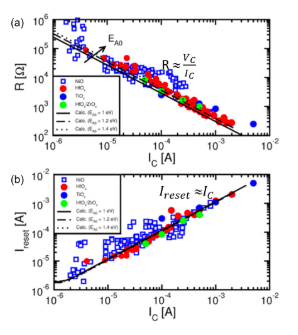
\includegraphics[width=2.5in]{fig9.png}
\caption{Dependence of the LRS resistance (top) and the RESET current (bottom) on the compliance current $I_\mathrm{CC}$ across several VCM oxide systems. $R_\mathrm{LRS}\!\propto\!V_c/I_\mathrm{CC}$ and $I_\mathrm{reset}\!\approx\!I_\mathrm{CC}$. Reproduced from~\cite{ref_ielmini2016}.}
\label{fig_icc}
\end{figure}

The second row constrains the off-state of the select FET. In a large array, every unselected cell sees a small bias and contributes a subthreshold leakage current; these add up across the array and degrade the read margin. The relevant figure of merit is the subthreshold swing $\mathrm{SS}=(kT/q)\ln 10\,(1+C_d/C_{ox})$, which sets how steeply $I_D$ falls below $V_T$. A steeper SS means more cells can share a wordline before the cumulative leakage corrupts a read; this is one of the main reasons FinFETs and FD-SOI MOSFETs (with smaller $C_d/C_{ox}$) are attractive hosts for RRAM at advanced nodes. DIBL is also constrained because it shifts $V_T$ at high $V_{DS}$, which would alter the saturation $I_D$ used to set $I_\mathrm{CC}$.

The third row is a co-optimization between the MOSFET and the BEOL. The on-resistance of the select MOSFET, $R_\mathrm{on}=L/[\mu_n C_{ox}\,W\,(V_{GS}-V_T)]$, must remain much smaller than $R_\mathrm{LRS}$, otherwise the read voltage divides between the cell and the transistor and the HRS/LRS distinction collapses.

\subsection{A Worked Example: Niu~2016 Planar Process}
Niu~\textit{et~al.} provide an explicit worked example of the sizing problem on a 0.25~$\mu$m planar CMOS line~\cite{ref_niu2016}. The cell is a HfO\textsubscript{2}/Ti/TiN MIM stack placed between metal~2 and metal~3 above an NMOS in the front-end. Starting from the series-circuit constraint
\begin{equation}
V_\mathrm{BL} \;=\; V_\mathrm{RRAM} + V_\mathrm{DS},
\end{equation}
and requiring the MOSFET to remain in saturation during forming and SET ($V_\mathrm{DS}>V_{GS}-V_T$), the design constraint becomes $V_\mathrm{BL}-V_\mathrm{SET}>V_{GS}-V_T$. Choosing $W=1.14~\mu$m and $L=0.24~\mu$m at $V_g=0.9$~V sets the saturation current to $I_\mathrm{CC}=10~\mu$A by Eq.~\eqref{eq:sizing}. The resulting LRS resistance is $R_\mathrm{LRS}=V_c/I_\mathrm{CC}=0.4~\mathrm{V}/10~\mu\mathrm{A}=40~\mathrm{k}\Omega$ (with $V_c\!\approx\!0.4$~V for HfO\textsubscript{2}), while the transistor on-resistance from the saturation model is $R_\mathrm{on}\!\approx\!200~\Omega$, comfortably below the 40~k$\Omega$ LRS as required by the read-margin constraint. Forming requires a higher voltage of 3.2--4.0~V on the bitline; the post-forming SET voltage falls to 0.8--1.1~V and RESET to 1.0--1.5~V~\cite{ref_niu2016}.

\begin{figure}[!t]
\centering
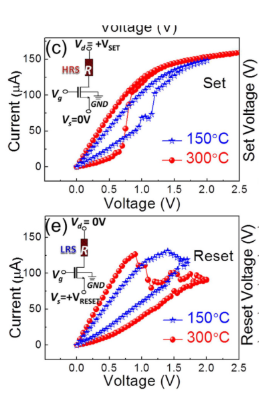
\includegraphics[width=2.4in]{fig10.png}
\caption{Measured $I$--$V$ characteristics of the integrated 1T1R HfO\textsubscript{2} cell from~\cite{ref_niu2016}, comparing two atomic layer deposition temperatures (150\,$^\circ$C in blue and 300\,$^\circ$C in red). Top:~SET; Bottom:~RESET. The 300\,$^\circ$C deposition produces tighter resistance distributions and lower switching voltages. Reproduced from~\cite{ref_niu2016}.}
\label{fig_niu_iv}
\end{figure}

The measured $I$--$V$ curves of this 1T1R cell, for two different ALD deposition temperatures, are shown in Fig.~\ref{fig_niu_iv}. Higher deposition temperature reduces residual carbon impurities from the metal-organic precursor and stabilizes the resistance distributions, lowering both $V_\mathrm{SET}$ and $V_\mathrm{RESET}$ and tightening cycle-to-cycle variability~\cite{ref_niu2016}. The case study makes the broader point that VCM RRAM electrical metrics are inseparable from process choices on the underlying materials stack.

\section{Technology-Dependent Challenges: Planar, FD-SOI, and FinFET}\label{sec:tech}
The same RRAM cell is integrated on top of three different MOSFET architectures in production today. Because the select-FET problem changes character with each architecture, the achievable cell density, $I_\mathrm{CC}$ control granularity, and forming headroom all change as well. Table~\ref{tab:arch} summarizes the comparison.

\begin{table}[!t]
\caption{Comparison of MOSFET Architectures Hosting RRAM\label{tab:arch}}
\centering
\footnotesize
\renewcommand{\arraystretch}{1.25}
\begin{tabular}{|p{0.85in}|p{0.6in}|p{0.6in}|p{0.6in}|}
\hline
\textbf{Parameter} & \textbf{Planar bulk} & \textbf{FD-SOI} & \textbf{FinFET} \\
\hline
$V_\mathrm{DD}$ & 1.0~V & 0.9--1.0~V & 0.8--0.9~V \\
\hline
$I_\mathrm{CC}$ control & $W/L$ + $V_g$ & $W/L$ + $V_g$ + back-gate & $N_\mathrm{fin}$ + $V_g$ \\
\hline
SS (mV/dec) & 80--100 & 65--75 & $\sim$65 \\
\hline
Min.\ cell area & 0.06~$\mu$m$^2$ & 0.066~$\mu$m$^2$ & 0.022~$\mu$m$^2$ \\
\hline
Forming headroom & OK & charge pump may be needed & charge pump required \\
\hline
Production eRRAM & TSMC 28~nm & STMicro / GF (22FDX) & TSMC 12~nm \\
\hline
\end{tabular}
\\[2pt]
\raggedright Adapted from~\cite{ref_ielmini2016} and~\cite{ref_hellenbrand2024}.
\end{table}

\textit{Planar bulk (250~nm down to 28~nm).} The starting point. Planar bulk MOSFETs offer continuous sizing of $W$ and $L$, which is the most flexible knob for tuning $I_\mathrm{CC}$. The penalty is the worst subthreshold slope of the three architectures (80--100~mV/dec), which limits the maximum array fan-out. TSMC's 40~nm and 28~nm embedded RRAM products are on planar bulk~\cite{ref_hellenbrand2024}, as is the Niu~2016 case study above.

\textit{FD-SOI (28FDSOI Samsung, 22FDX GlobalFoundries).} The fully-depleted silicon-on-insulator transistor adds a back-gate that can be biased independently of the front gate. In the 1T1R cell this back-gate provides per-die threshold trim of the select FET, which translates into per-die $I_\mathrm{CC}$ trim---useful for compensating both the process variation in the FET and the much larger device-to-device variation in the RRAM cell itself. The subthreshold slope improves to 65--75~mV/dec because the buried oxide effectively eliminates the body capacitance term $C_d$. The trade-off is a slightly larger minimum cell area and a marginal forming headroom, since $V_\mathrm{DD}$ is similar to or below the planar value while the forming voltage at the cell remains near 3~V. Weebit~Nano's TaO\textsubscript{x} ReRAM IP has been integrated into the 22FDX FD-SOI platform~\cite{ref_hellenbrand2024}.

\textit{FinFET (16~nm and below).} The FinFET delivers the steepest subthreshold slope of any production architecture ($\sim$65~mV/dec), which raises the achievable array fan-out, and provides higher drive current per footprint, which helps deliver $I_\mathrm{CC}$ in a small cell. The cell area is the smallest of the three, at roughly 0.022~$\mu$m$^2$. The trade-off is geometric: $W$ is no longer continuous but quantized into integer fins. Sizing for a target $I_\mathrm{CC}$ may force rounding to the next fin count, which shows up as a granular $I_\mathrm{CC}$ ladder rather than a smooth one. In addition, the lower $V_\mathrm{DD}$ (0.8--0.9~V) leaves less headroom to deliver the forming voltage at the cell, which makes a dedicated charge pump effectively mandatory. TSMC presented an embedded RRAM macro on its 12~nm FinFET technology at IEDM~2023~\cite{ref_hellenbrand2024}.

\begin{figure}[!t]
\centering
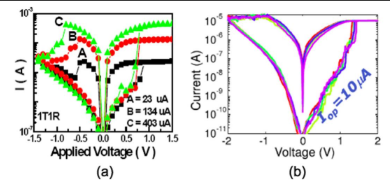
\includegraphics[width=3.4in]{fig11.png}
\caption{Measured $I$--$V$ characteristics of an integrated 1T1R HfO\textsubscript{x} cell at three compliance current levels (a), and the resulting LRS/HRS distributions versus operating compliance (b). The compliance current is set by the select MOSFET. Reproduced from~\cite{ref_ielmini2016}.}
\label{fig_iv_family}
\end{figure}

The dependence of the cell electrical characteristics on $I_\mathrm{CC}$, common to all three architectures, is shown in Fig.~\ref{fig_iv_family}. The select MOSFET sets the compliance, and the LRS resistance, RESET current, and read margin all track it. The architectural choice therefore matters not only for area and array size but for the achievable granularity of the $I_\mathrm{CC}$ knob---continuous on planar bulk, continuously trimmable on FD-SOI, and quantized on FinFET.

\section{Conclusion}\label{sec:conclusion}
Resistive RAM is now the standard embedded non-volatile memory at logic nodes that have outgrown floating-gate flash. Its commercial success rests on three foundations: a simple two-terminal MIM cell of materials already qualified in CMOS fabrication; a back-end-of-line integration that leaves the front-end logic essentially unchanged; and the 1T1R cell architecture in which a CMOS select MOSFET handles current limiting, addressing, and isolation. The dominant operating mechanism is the valence-change family of HfO\textsubscript{x} and TaO\textsubscript{x} cells, in which oxygen-vacancy migration creates and disconnects a filamentary conductive path.

The MOSFET-modeling content of the technology is concentrated in the select FET, whose sizing maps the RRAM compliance current $I_\mathrm{CC}$ onto a $W/L$ design through the saturation current model, and whose subthreshold characteristics set the maximum achievable array size through cumulative sneak leakage. The Niu~2016 case study on a 0.25~$\mu$m planar process shows the sizing problem in its simplest continuous form. Moving to FD-SOI adds a back-gate that gives per-die $I_\mathrm{CC}$ trim; moving to FinFET drops the cell area and the subthreshold slope but quantizes the sizing knob and tightens the forming headroom. Each architectural step on the MOSFET roadmap reshapes the select-FET problem rather than eliminating it, which is why RRAM remains an active integration target as logic continues to scale.

\begin{thebibliography}{1}
\bibliographystyle{IEEEtran}

\bibitem{ref_wong2012}
H.-S.\ P.\ Wong, H.-Y.\ Lee, S.\ Yu, Y.-S.\ Chen, Y.\ Wu, P.-S.\ Chen, B.\ Lee, F.\ T.\ Chen, and M.-J.\ Tsai, ``Metal--oxide RRAM,'' \textit{Proc.\ IEEE}, vol.\ 100, no.\ 6, pp.\ 1951--1970, Jun.\ 2012, doi:~10.1109/JPROC.2012.2190369.

\bibitem{ref_waser2009}
R.\ Waser, R.\ Dittmann, G.\ Staikov, and K.\ Szot, ``Redox-based resistive switching memories---nanoionic mechanisms, prospects, and challenges,'' \textit{Adv.\ Mater.}, vol.\ 21, no.\ 25--26, pp.\ 2632--2663, Jul.\ 2009, doi:~10.1002/adma.200900375.

\bibitem{ref_ielmini2016}
D.\ Ielmini, ``Resistive switching memories based on metal oxides: mechanisms, reliability and scaling,'' \textit{Semicond.\ Sci.\ Technol.}, vol.\ 31, no.\ 6, art.\ 063002, May~2016, doi:~10.1088/0268-1242/31/6/063002.

\bibitem{ref_niu2016}
G.\ Niu, H.-D.\ Kim, R.\ Roelofs, E.\ Perez, M.\ A.\ Schubert, P.\ Zaumseil, I.\ Costina, and C.\ Wenger, ``Material insights of HfO\textsubscript{2}-based integrated 1-transistor--1-resistor resistive random access memory devices processed by batch atomic layer deposition,'' \textit{Sci.\ Reports}, vol.\ 6, art.\ 28155, Jun.\ 2016, doi:~10.1038/srep28155.

\bibitem{ref_hellenbrand2024}
M.\ Hellenbrand, I.\ Teck, and J.\ L.\ MacManus-Driscoll, ``Progress of emerging non-volatile memory technologies in industry,'' \textit{MRS Commun.}, vol.\ 14, no.\ 6, pp.\ 1099--1112, Nov.\ 2024, doi:~10.1557/s43579-024-00660-2.

\end{thebibliography}

\end{document}
